\documentclass[main.tex]{subfiles}
\begin{document}\newpage
\setdoublesep{0.35700 em}  % 'Bond Spacing'
\setatomsep{1.78500 em}    % 'Fixed Length'
\setbondoffset{0.18265 em} % 'Margin Width'
\newcommand{\bondwidth}{0.06642 em} % 'Line Width'
\setbondstyle{line width = \bondwidth}
\newgeometry{left=0.8in,right=0.8in, top=2.5cm,bottom=2cm}
\fancyhfoffset[E,O]{0pt}
\setlength{\columnsep}{30pt}
\begin{conclusion}
\end{conclusion}
%\setstretch{0.3}
\begin{multicols*}{2}\setcounter{numA}{1}



{\raggedright\textsc{\textbf{Rate of reaction }}\par}
%%%%%%PROBLEM
%\begin{question}[ID=\the\value{numA}]\SetQuestionProperties{section-title=\nameref{sec:units}}
%For the following colloids, indicate the nature (liquid, solid or gad) of the dispersed and dispersing medium: 
%\begin{inparaenum}[(a)]	
%\item  soda water % (dispersed: gas ; dispersing: liquid)
%\item  cake % (dispersed: gas ; dispersing: solid)
%\item  midst % (dispersed: liquid ; dispersing: gas)
%\item  smoke % (dispersed: solid ; dispersing: gas)
%\item  froth % (dispersed: gas ; dispersing: liquid)
% \end{inparaenum}
%\end{question}
%\begin{solution}
%\begin{inparaenum}[(a)]
%\item  soda water   (dispersed: gas ; dispersing: liquid)
%\item  cake   (dispersed: gas ; dispersing: solid)
%\item  midst   (dispersed: liquid ; dispersing: gas)
%\item  smoke   (dispersed: solid ; dispersing: gas)
%\item  froth   (dispersed: gas ; dispersing: liquid)
% \end{inparaenum}
%\hspace{0.1cm}\end{solution}\stepcounter{numA}%%%%%%%%%%%%




%%%%%%PROBLEM
\begin{question}[ID=\the\value{numA}]\SetQuestionProperties{section-title=\nameref{sec:units}}
A is the reactant of two different reactions. Plot the data below in order to compare the rate of the two reaction.
\begin{center}\begin{tabular}[t]{  c c  c c     }
\toprule
 &Reaction I&		Reaction II	 \\
\toprule
Time, s	&	$[A]$ (M)	&		$[A]$ (M)	 \\
\midrule
0&	100	&	100	\\
1&	$7\times 10^{-1}$	&	36.78	\\
2&	$4\times 10^{-3}$	&	13.53	\\
3&	$3\times 10^{-5}$	&	4.90	\\
4&	$2\times 10^{-7}$	&	1.80	\\
\bottomrule
\end{tabular}\end{center}
\end{question}
\begin{solution}
Reaction I is faster
\hspace{0.1cm}\end{solution}\stepcounter{numA}%%%%%%%%%%%%


%%%%%%PROBLEM
\begin{question}[ID=\the\value{numA}]\SetQuestionProperties{section-title=\nameref{sec:units}}
Use the data below to identify reactants and products in a reaction.
\begin{center}\begin{tabular}[t]{  c c  c c     }
\toprule
Time, s	&	$[A]$ (M)	&		$[B]$ (M)	 \\
\midrule
0&	0&	3		\\
1	&	$2\times 10^{-2}$&	$2.4 $	\\
2	&	$3\times 10^{-2}$	&	$2.0 $\\
3&	$6\times 10^{-2}$&	$1.64 $		\\
4&	$8\times 10^{-2}$&	$1.34 $		\\
\bottomrule
\end{tabular}\end{center}
\end{question}
\begin{solution}
B is the reactants and A the product
\hspace{0.1cm}\end{solution}\stepcounter{numA}%%%%%%%%%%%%


%%%%%%PROBLEM
\begin{question}[ID=\the\value{numA}]\SetQuestionProperties{section-title=\nameref{sec:units}}
Use the data below to identify reactants and products in a reaction.
\begin{center}\begin{tabular}[t]{  c c  c c     }
\toprule
Time, s	&	$[A]$ (M)	&		$[B]$ (M)	 \\
\midrule
0&	2	&	0	\\
1&	$1.996 $	&	$4\times 10^{-3}$	\\
2&	$1.992 $	&	$8\times 10^{-3}$	\\
3&	$1.988 $	&	$1.2\times 10^{-2}$	\\
4&	$1.984 $	&	$1.6\times 10^{-2}$	\\
\bottomrule
\end{tabular}\end{center}
\end{question}
\begin{solution}
A is the reactants and B the product
\hspace{0.1cm}\end{solution}\stepcounter{numA}%%%%%%%%%%%%



%%%%%%PROBLEM
\begin{question}[ID=\the\value{numA}]\SetQuestionProperties{section-title=\nameref{sec:units}}
Use the data below to identify reactants and products in a reaction.
\begin{center}\begin{tabular}[t]{  c c  c c     }
\toprule
Time, s	&	$[A]$ (M)	&		$[B]$ (M)	 \\
\midrule
0&	4	&	0	\\
1&	$3.6 $	&	$2\times 10^{-3}$	\\
2&	$2.2 $	&	$2\times 10^{-3}$	\\
3&	$1.3 $	&	$2\times 10^{-2}$	\\
4&	$0.8 $	&	$2\times 10^{-2}$	\\
\bottomrule
\end{tabular}\end{center}
\end{question}
\begin{solution}
A is the reactants and B neither reactant or product
\hspace{0.1cm}\end{solution}\stepcounter{numA}%%%%%%%%%%%%


%%%%%%PROBLEM
\begin{question}[ID=\the\value{numA}]\SetQuestionProperties{section-title=\nameref{sec:units}}
The concentration plots below represent two different reaction. Indicate which has the fastest initial reaction rate.\\
\begin{adjustbox}{width={8cm},totalheight={6cm},keepaspectratio}
  
    \pgfkeys{tikz/.cd,
tangent length/.store in=\TangentLength,
tangent length=7mm,
normal length/.store in=\NormalLength,
normal length=7mm}
\tikzset{tangent/.style={red,thin},normal/.style={red,thin},
tangent at/.style={postaction={decorate,decoration={markings,
mark=at position #1 with {\draw[tangent,shift={(0,1.60em-1.6em)}, rotate=-0] (-2*\TangentLength,0) -- (0.4*\TangentLength,0)   -- ++ (-4.7em,-0.6em) -- cycle; \node[shift={(-2em,1em)}, red] (-\TangentLength,0) {$r$} node[shift={(-4.4em,.3em)}, red] (-\TangentLength,0) {\tiny $d$c} node[shift={(-2em,-.2em)}, red] (-\TangentLength,0) {\tiny $d$t};
\fill[tangent,shift={(0,1.60em-1.6em)}]  (-\TangentLength,0) circle (1pt);}}}},
%normal at/.style={postaction={decorate,decoration={markings,
%mark=at position #1 with {\draw[normal] (0,-\NormalLength) -- (0,\NormalLength);
%\fill[normal] (0,0) circle (2pt);}}}},
}
\begin{tikzpicture}
  \begin{axis}[
            axis lines=middle,
             enlargelimits=0.1,
            xmin=0,
            xmax=1.0,
            ymin=0.01,
            ymax=0.1,
            xtick=\empty,
            ytick=\empty,xtick distance=0.05,
            xlabel=$\text{time}$,
            ylabel=$A\text{, M}$,
            x label style={at={(axis description cs:0.5,-0.0)},anchor=north},
    y label style={at={(axis description cs:0.07,.4)},rotate=90,anchor=south},
             domain=\pgfkeysvalueof{/pgfplots/xmin}:(\pgfkeysvalueof{/pgfplots/xmax},
            tangent/.style={add node at x={#1}{},},
        ]
     	              %, tangent at/.list={ 0.8 }
            \addplot [thick,draw=blue!75!black   ]{0.1*exp(-2.9*x)};
%                         \addplot [blue!75!black, mark=*,  draw=none , samples=5 ]{0.1*exp(-2.9*x)};
%	 \draw[red] (6.4em,6em+0.8em) --++(0em,-3.5em+0.1em)--++(6.1em,0em ) -- cycle ;
%                \addplot  [thick,draw=green!75!black]{0.1*(1-exp(-2.9*x))};
%	             \addplot  [green!75!black, mark=*,  draw=none , samples=5]{0.1*(1-exp(-2.9*x))}; 


        \end{axis}\end{tikzpicture} 
        \begin{tikzpicture}

          \begin{axis}[
            axis lines=middle,
             enlargelimits=0.1,
            xmin=0,
            xmax=1.0,
            ymin=0.01,
            ymax=0.1,
            xtick=\empty,
            ytick=\empty,xtick distance=0.05,
            xlabel=$\text{time}$,
            ylabel=$A\text{, M}$,
            x label style={at={(axis description cs:0.5,-0.0)},anchor=north},
    y label style={at={(axis description cs:0.07,.4)},rotate=90,anchor=south},
             domain=\pgfkeysvalueof{/pgfplots/xmin}:(\pgfkeysvalueof{/pgfplots/xmax},
            tangent/.style={add node at x={#1}{},},
        ]
     	              %, tangent at/.list={ 0.8 }
            \addplot [thick,draw=blue!75!black   ]{0.1*exp(-9*x)};
%                         \addplot [blue!75!black, mark=*,  draw=none , samples=5 ]{0.1*exp(-2.9*x)};
%	 \draw[red] (6.4em,6em+0.8em) --++(0em,-3.5em+0.1em)--++(6.1em,0em ) -- cycle ;
%                \addplot  [thick,draw=green!75!black]{0.1*(1-exp(-2.9*x))};
%	             \addplot  [green!75!black, mark=*,  draw=none , samples=5]{0.1*(1-exp(-2.9*x))}; 


        \end{axis}

\end{tikzpicture} 
 \end{adjustbox} 
\end{question}
\begin{solution}
The plot on the right
\hspace{0.1cm}\end{solution}\stepcounter{numA}%%%%%%%%%%%%


%%%%%%PROBLEM
\begin{question}[ID=\the\value{numA}]\SetQuestionProperties{section-title=\nameref{sec:units}}
Using the concentration vs. time plot shown below, compare the instantaneous rate at both different times.\\
\begin{adjustbox}{width={8cm},totalheight={6cm},keepaspectratio}
  
    \pgfkeys{tikz/.cd,
tangent length/.store in=\TangentLength,
tangent length=7mm,
normal length/.store in=\NormalLength,
normal length=7mm}
\tikzset{tangent/.style={red,thin},normal/.style={red,thin},
tangent at/.style={postaction={decorate,decoration={markings,
mark=at position #1 with {\draw[tangent,shift={(0,1.5em )}, rotate=-0] (-2*\TangentLength,0) -- (0.4*\TangentLength,0) ;
%  -- ++ (-4.7em,-0.6em) -- cycle; 
%\node[shift={(-2em,1em)}, red] (-\TangentLength,0) {$r$} node[shift={(-4.4em,.3em)}, red] (-\TangentLength,0) {\tiny $d$c} node[shift={(-2em,-.2em)}, red] (-\TangentLength,0) {\tiny $d$t};
\fill[tangent,shift={(0,1.5em )}]  (-0.9*\TangentLength,0) circle (1pt)   ;}}	}},
%normal at/.style={postaction={decorate,decoration={markings,
%mark=at position #1 with {\draw[normal] (0,-\NormalLength) -- (0,\NormalLength);
%\fill[normal] (0,0) circle (2pt);}}}},
}
\begin{tikzpicture}
  \begin{axis}[
            axis lines=middle,
             enlargelimits=0.1,
            xmin=0,
            xmax=1.0,
            ymin=0.01,
            ymax=0.1,
            xtick=\empty,
            ytick=\empty,xtick distance=0.05,
            xlabel=$\text{time}$,
            ylabel=$A\text{, M}$,
            x label style={at={(axis description cs:0.5,-0.0)},anchor=north},
    y label style={at={(axis description cs:0.07,.4)},rotate=90,anchor=south},
             domain=\pgfkeysvalueof{/pgfplots/xmin}:(\pgfkeysvalueof{/pgfplots/xmax},
            tangent/.style={add node at x={#1}{},},
        ]
     	              %, tangent at/.list={ 0.8 }
            \addplot [thick,draw=blue!75!black, tangent at/.list={ 0.8  },tangent at/.list={ 0.3  }   ]{0.1*exp(-2.9*x)};
%                         \addplot [blue!75!black, mark=*,  draw=none , samples=5 ]{0.1*exp(-2.9*x)};
%	 \draw[red] (6.4em,6em+0.8em) --++(0em,-3.5em+0.1em)--++(6.1em,0em ) -- cycle ;
%                \addplot  [thick,draw=green!75!black]{0.1*(1-exp(-2.9*x))};
%	             \addplot  [green!75!black, mark=*,  draw=none , samples=5]{0.1*(1-exp(-2.9*x))}; 


        \end{axis}\end{tikzpicture} 
 
 \end{adjustbox} 
\end{question}
\begin{solution}
$r_{left}$>$r_{right}$
\hspace{0.1cm}\end{solution}\stepcounter{numA}%%%%%%%%%%%%





%%%%%%PROBLEM
\begin{question}[ID=\the\value{numA}]\SetQuestionProperties{section-title=\nameref{sec:units}}
Using the concentration vs. time plot shown below, compare the instantaneous rate at both different times.\\
\begin{adjustbox}{width={8cm},totalheight={6cm},keepaspectratio}
  
    \pgfkeys{tikz/.cd,
tangent length/.store in=\TangentLength,
tangent length=7mm,
normal length/.store in=\NormalLength,
normal length=7mm}
\tikzset{tangent/.style={red,thin},normal/.style={red,thin},
tangent at/.style={postaction={decorate,decoration={markings,
mark=at position #1 with {\draw[tangent,shift={(0,-0.1em )}, rotate=-0] (-2*\TangentLength,0) -- (0.4*\TangentLength,0) ;
%  -- ++ (-4.7em,-0.6em) -- cycle; 
%\node[shift={(-2em,1em)}, red] (-\TangentLength,0) {$r$} node[shift={(-4.4em,.3em)}, red] (-\TangentLength,0) {\tiny $d$c} node[shift={(-2em,-.2em)}, red] (-\TangentLength,0) {\tiny $d$t};
\fill[tangent,shift={(0,-0.1em )}]  (-0.5*\TangentLength,0) circle (1pt)   ;}}	}},
%normal at/.style={postaction={decorate,decoration={markings,
%mark=at position #1 with {\draw[normal] (0,-\NormalLength) -- (0,\NormalLength);
%\fill[normal] (0,0) circle (2pt);}}}},
}
\begin{tikzpicture}
  \begin{axis}[
            axis lines=middle,
             enlargelimits=0.1,
             xmin=0,
             xmax=10.0,
             ymin=0.01,
             ymax=3.1,
            xtick=\empty,
            ytick=\empty,xtick distance=0.05,
            xlabel=$\text{time}$,
            ylabel=$A\text{, M}$,
            x label style={at={(axis description cs:0.5,-0.0)},anchor=north},
    y label style={at={(axis description cs:0.07,.4)},rotate=90,anchor=south},
             domain=\pgfkeysvalueof{/pgfplots/xmin}:(\pgfkeysvalueof{/pgfplots/xmax},
            tangent/.style={add node at x={#1}{},},
        ]
     	              %, tangent at/.list={ 0.8 }
            \addplot [thick,draw=blue!75!black, tangent at/.list={ 0.8  },tangent at/.list={ 0.3  }   ]{ln(x)/ln(3)+.8};
%                         \addplot [blue!75!black, mark=*,  draw=none , samples=5 ]{0.1*exp(-2.9*x)};
%	 \draw[red] (6.4em,6em+0.8em) --++(0em,-3.5em+0.1em)--++(6.1em,0em ) -- cycle ;
%                \addplot  [thick,draw=green!75!black]{0.1*(1-exp(-2.9*x))};
%	             \addplot  [green!75!black, mark=*,  draw=none , samples=5]{0.1*(1-exp(-2.9*x))}; 


        \end{axis}\end{tikzpicture} 
 
 \end{adjustbox} 
\end{question}
\begin{solution}
$r_{left}$>$r_{right}$
\hspace{0.1cm}\end{solution}\stepcounter{numA}%%%%%%%%%%%%


%%%%%%PROBLEM
\begin{question}[ID=\the\value{numA}]\SetQuestionProperties{section-title=\nameref{sec:units}}
For a given reaction the differential rate is measured for a set of species. Given the numerical values indicated next, identify the specie as reactant or product:
\begin{inparaenum}[(a)]
\item  $r_A$=0.3M/s  % (product)
\item  $r_B$=-0.1M/s  % (reactant)
\item  $r_C$=-1.2M/s  % (reactant)
\item  $r_D$=0.6M/s  % (product)
\end{inparaenum}
\end{question}
\begin{solution}
\begin{inparaenum}[(a)]
\item  $r_A$=0.3M/s    (product)
\item  $r_B$=-0.1M/s    (reactant)
\item  $r_C$=-1.2M/s    (reactant)
\item  $r_D$=0.6M/s    (product)
\end{inparaenum}\hspace{0.1cm}\end{solution}\stepcounter{numA}%%%%%%%%%%%%

%%%%%%PROBLEM
\begin{question}[ID=\the\value{numA}]\SetQuestionProperties{section-title=\nameref{sec:units}}
For the reaction below: \ce{2a	+	3b	->	4c	+	5d }
and given that the rate of disappearance of b is $r_B$=-0.3M/s, calculate:
\begin{inparaenum}[(a)]
\item  the rate of disappearance of A, $r_A$   % (- 0.2M/s)
\item  the rate of appearance of C, $r_C$   % (+0.4M/s )
\item  the rate of appearance of D, $r_D$   % (+0.5M/s )
\item  the rate of reaction $r$   % (0.1M/s )
\end{inparaenum}
\end{question}
\begin{solution}
\begin{inparaenum}[(a)]
\item   - 0.2M/s
\item   +0.4M/s 
\item    +0.5M/s 
\item    0.1M/s
\end{inparaenum}\hspace{0.1cm}\end{solution}\stepcounter{numA}%%%%%%%%%%%%

      
%%%%%%PROBLEM
\begin{question}[ID=\the\value{numA}]\SetQuestionProperties{section-title=\nameref{sec:units}}
For the reaction below: \ce{2a	+	2b -> 3c	+	d            }
and given that the rate of appearance of d is $r_D$=0.2M/s, calculate:
\begin{inparaenum}[(a)]
\item  the rate of disappearance of A, $r_A$   % (- 0.4M/s)
\item  the rate of disappearance of B, $r_B$   % (- 0.4M/s)
\item  the rate of appearance of C, $r_C$   % (+0.6M/s )
\item  the rate of reaction $r$   % (0.2M/s )
\end{inparaenum}
\end{question}
\begin{solution}
\begin{inparaenum}[(a)]
\item    - 0.4M/s
\item    - 0.4M/s
\item    +0.6M/s 
\item    0.2M/s
\end{inparaenum}\hspace{0.1cm}\end{solution}\stepcounter{numA}%%%%%%%%%%%%



{\raggedright\textsc{\textbf{Rate laws }}\par}

%%%%%%PROBLEM
\begin{question}[ID=\the\value{numA}]\SetQuestionProperties{section-title=\nameref{sec:units}}
Given the following rate law
\begin{center}$r$=0.04[A]$^2$[B][C]$^3$\end{center}
indicate:
\begin{inparaenum}[(a)]
\item  the reaction order of A  % (second order)
\item  the reaction order of B  % (first order)
\item  the reaction order of C  % (third order)
\item  the overall reaction order% (sixth order)
\item  the value of the reaction constant including its units  % (0.04 s/M$^5$)
\end{inparaenum}
\end{question}
\begin{solution}
\begin{inparaenum}[(a)]
\item   second order
\item   first order
\item   third order
\item   sixth order
\item   0.04 s/M$^5$
\end{inparaenum}\hspace{0.1cm}\end{solution}\stepcounter{numA}%%%%%%%%%%%%


%%%%%%PROBLEM
\begin{question}[ID=\the\value{numA}]\SetQuestionProperties{section-title=\nameref{sec:units}}
Given the following rate law
\begin{center}$r$=0.4[\ce{Cl2}][\ce{F2}]$^2$\end{center}
indicate:
\begin{inparaenum}[(a)]
\item  the reaction order of \ce{Cl2}  % (first order)
\item  the reaction order of \ce{F2}  % (second order)
\item  the overall reaction order% (third order)
\item  the value of the reaction constant including its units  % (0.4 s/M$^2$)
\end{inparaenum}
\end{question}
\begin{solution}
\begin{inparaenum}[(a)]
\item   first order
\item   second order
\item   third order
\item   0.4 s/M$^2$
\end{inparaenum}\hspace{0.1cm}\end{solution}\stepcounter{numA}%%%%%%%%%%%%



%%%%%%PROBLEM
\begin{question}[ID=\the\value{numA}]\SetQuestionProperties{section-title=\nameref{sec:units}}
Given the following rate law
\begin{center}$r$=k[A]$^4$[B]$^2$[C]$^2$\end{center}
indicate the impact on the rate of the following:
\begin{inparaenum}[(a)]
\item  to double [A]  % ( 16 times faster)
\item  to triple [B]  % ( 9 times faster)
\item  to double [C]% ( 4 times faster)
\end{inparaenum}
\end{question}
\begin{solution}
\begin{inparaenum}[(a)]
\item    16 times faster 
\item    9 times faster  
\item    4 times faster 
\end{inparaenum}\hspace{0.1cm}\end{solution}\stepcounter{numA}%%%%%%%%%%%%

%%%%%%PROBLEM
\begin{question}[ID=\the\value{numA}]\SetQuestionProperties{section-title=\nameref{sec:units}}
Given the following rate law
\begin{center}$r$=k[A][B]$^2$[C]\end{center}
indicate the impact on the rate of the following:
\begin{inparaenum}[(a)]
\item  to double [B]  % ( 4 times faster)
\item  to triple [A]  % (3 times faster)
\item  to quadruple [C]% ( 4 times faster)
\end{inparaenum}
\end{question}
\begin{solution}
\begin{inparaenum}[(a)]
\item  4 times faster
\item   3 times faster 
\item   4 times faster 
\end{inparaenum}\hspace{0.1cm}\end{solution}\stepcounter{numA}%%%%%%%%%%%%


%%%%%%PROBLEM
\begin{question}[ID=\the\value{numA}]\SetQuestionProperties{section-title=\nameref{sec:units}}
Given the following rate constant values, identify the reaction order:
\begin{inparaenum}[(a)]

\item  k=$3\times 10^{-4}$ L/(s$\cdot$mol) % (second order)
\item k=0.03 M/s % (zeroth order)
\item  k=$3\times 10^{-5}$ 1/(s$\cdot$M$^2$) % (third order)
\end{inparaenum}
\end{question}
\begin{solution}
\begin{inparaenum}[(a)]

\item   second order 
\item  zeroth order 
\item   third order 
\end{inparaenum}\hspace{0.1cm}\end{solution}\stepcounter{numA}%%%%%%%%%%%%
	    	         
                 
   %%%%%%PROBLEM
\begin{question}[ID=\the\value{numA}]\SetQuestionProperties{section-title=\nameref{sec:units}}
Given the following rate constant values, identify the reaction order:
\begin{inparaenum}[(a)]
\item  k=0.04 M/s  	% ( zeroth order)
\item   k=0.00 1/s 	% (first order)
\item  k=0.09 s/M	% (second order)

\end{inparaenum}
\end{question}
\begin{solution}
\begin{inparaenum}[(a)]
\item    zeroth order 
\item    first order 
\item   second order 
\end{inparaenum}\hspace{0.1cm}\end{solution}\stepcounter{numA}%%%%%%%%%%%%             


   %%%%%%PROBLEM
\begin{question}[ID=\the\value{numA}]\SetQuestionProperties{section-title=\nameref{sec:units}}
Identify the following rate laws as integral or differential, and given a form obtain the corresponding other type of from (i.e. if the integral from is given then obtain the differential form)
\begin{inparaenum}[(a)]
\item 	  $r=0.0023$, $[A]_0$=0.3  	%	(differential, $ [\ce{A}] =-0.0023\cdot t + 0.3$)
\item $Ln([\ce{A}])=-0.045\cdot t+0.45$	%	(integral, $r=0.045[A]^1$, $[A]_0$=1.56)
\item 	   $r=0.3[A]^2$, $[A]_0$=25   	%	(differential, $\frac{1}{[\ce{A}]}=0.3\cdot t +0.04$)
\end{inparaenum}
\end{question}
\begin{solution}
\begin{inparaenum}[(a)]
\item 	  $r=0.0023$, $[A]_0$=0.3  	%	(differential, $ [\ce{A}] =-0.0023\cdot t + 0.3$)
\item $Ln([\ce{A}])=-0.045\cdot t+0.45$	%	(integral, $r=0.045[A]^1$, $[A]_0$=1.56)
\item 	   $r=0.3[A]^2$, $[A]_0$=25   	%	(differential, $\frac{1}{[\ce{A}]}=0.3\cdot t +0.04$)
\end{inparaenum}\hspace{0.1cm}\end{solution}\stepcounter{numA}%%%%%%%%%%%% 


   %%%%%%PROBLEM
\begin{question}[ID=\the\value{numA}]\SetQuestionProperties{section-title=\nameref{sec:units}}
Identify the following rate laws as integral or differential, and given a form obtain the corresponding other type of from (i.e. if the integral from is given then obtain the differential form)
\begin{inparaenum}[(a)]

\item $[\ce{A}] =0.045 -0.34\cdot t $	 	%	(integral, $r=0.34$, $[A]_0$=0.045)
\item 	   $r=0.9[A]^1$, $[A]_0$=1.49   %	(differential, $Ln([\ce{A}])=0.4 -0.9\cdot t$)
\item $\frac{1}{[\ce{A}]}=0.3+0.04\cdot t $	%	(integral, $r=0.04[A]^2$, $[A]_0$=3.33)
\end{inparaenum}
\end{question}
\begin{solution}
\begin{inparaenum}[(a)]

\item $[\ce{A}] =0.045 -0.34\cdot t $	 	%	(integral, $r=0.34$, $[A]_0$=0.045)
\item 	   $r=0.9[A]^1$, $[A]_0$=1.49   %	(differential, $Ln([\ce{A}])=0.4 -0.9\cdot t$)
\item $\frac{1}{[\ce{A}]}=0.3+0.04\cdot t $	%	(integral, $r=0.04[A]^2$, $[A]_0$=3.33)
\end{inparaenum}\hspace{0.1cm}\end{solution}\stepcounter{numA}%%%%%%%%%%%%  


   %%%%%%PROBLEM
\begin{question}[ID=\the\value{numA}]\SetQuestionProperties{section-title=\nameref{sec:units}}
Compute the half-life for the following reactions:
\begin{inparaenum}[(a)]
\item a first order reaction with $k$=0.234 1/s	 	%	(2.96s)
\item a zeroth-order reaction with $k$=0.34 M/s	 and initial concentration 0.1M	%	(0.15 s)
\item a second-order reaction with $k$=0.067 M/s	 and initial concentration 0.01M	%	(1492 s)
\end{inparaenum}
\end{question}
\begin{solution}
\begin{inparaenum}[(a)]
\item  2.96s 
\item  0.15 s
\item  1492 s
\end{inparaenum}\hspace{0.1cm}\end{solution}\stepcounter{numA}%%%%%%%%%%%%  




{\raggedright\textsc{\textbf{The differential and integral methods of obtaining rate laws }}\par}


%%%%%%PROBLEM
\begin{question}[ID=\the\value{numA}]\SetQuestionProperties{section-title=\nameref{sec:units}}
Use the data below to calculate the rate law of the following reaction: \begin{center}\ce{A -> B}\end{center}
\begin{center}\begin{tabular}[t]{  c c  c   }
\toprule
 Experiment &$r$ (M/s)	&$[A]$, (M) \\
\midrule
1&	0.03&	1\\
2&	0.12 &2	\\
\bottomrule
\end{tabular}\end{center}
\end{question}
\begin{solution}
$r=0.03[A]^2$
\hspace{0.1cm}\end{solution}\stepcounter{numA}%%%%%%%%%%%%  


%%%%%%PROBLEM
\begin{question}[ID=\the\value{numA}]\SetQuestionProperties{section-title=\nameref{sec:units}}
Use the data below to calculate the rate law of the following reaction: \begin{center}\ce{A -> B}\end{center}
\begin{center}\begin{tabular}[t]{  c c  c   }
\toprule
 Experiment &$r$ (M/s)	&$[A]$, (M) \\
\midrule
1&	$5\times 10^{-3}$&	0.5\\
2&	$5\times 10^{-3}$ &0.6	\\
\bottomrule
\end{tabular}\end{center}
\end{question}
\begin{solution}
$r=0.005$
\hspace{0.1cm}\end{solution}\stepcounter{numA}%%%%%%%%%%%%  


%%%%%%PROBLEM
\begin{question}[ID=\the\value{numA}]\SetQuestionProperties{section-title=\nameref{sec:units}}
Use the data below to calculate the rate law of the following reaction: \begin{center}\ce{A -> B}\end{center}
\begin{center}\begin{tabular}[t]{  c c  c   }
\toprule
 Experiment &$r$ (M/s)	&$[A]$, (M) \\
\midrule
1&	0.03&	0.1\\
2&	0.30 &0.2	\\
\bottomrule
\end{tabular}\end{center}
\end{question}
\begin{solution}
$r=0.15[A]$
\hspace{0.1cm}\end{solution}\stepcounter{numA}%%%%%%%%%%%%  

%%%%%%PROBLEM
\begin{question}[ID=\the\value{numA}]\SetQuestionProperties{section-title=\nameref{sec:units}}
Use the data below to calculate the rate law:
\begin{center}\begin{tabular}[t]{  c c  c c  c  }
\toprule
Experiment	&$[A]$ (M)&		$[B]$ (M)	&	$r$ (M/s)\\
\midrule
1&	0.1&	0.02&	$2.08\times 10^{-5}$\\
2&	0.1&	0.04&	$8.32\times 10^{-5}$\\
3&	0.2&	0.01&	$1.04\times 10^{-5}$\\
4&	0.4	&0.01	&$2.08\times 10^{-5}$\\
\bottomrule
\end{tabular}\end{center}
\end{question}
\begin{solution}
$r=0.52[A]^1[B]^2$
\hspace{0.1cm}\end{solution}\stepcounter{numA}%%%%%%%%%%%%  

%%%%%%PROBLEM
\begin{question}[ID=\the\value{numA}]\SetQuestionProperties{section-title=\nameref{sec:units}}
Use the data below to calculate the rate law:
\begin{center}\begin{tabular}[t]{  c c  c c  c  }
\toprule
Experiment	&$[A]$ (M)&		$[B]$ (M)	&	$r$ (M/s)\\
\midrule
1&	0.1&	0.02&	$1.03\times 10^{-3}$\\
2&	0.1&	0.04&	$2.08\times 10^{-3}$\\
3&	0.2&	0.01&	$1.04\times 10^{-3}$\\
4&	0.4	&0.01	&$2.08\times 10^{-3}$\\
\bottomrule
\end{tabular}\end{center}
\end{question}
\begin{solution}
$r=0.52[A][B]$
\hspace{0.1cm}\end{solution}\stepcounter{numA}%%%%%%%%%%%%  



%%%%%%PROBLEM
\begin{question}[ID=\the\value{numA}]\SetQuestionProperties{section-title=\nameref{sec:units}}
Use the data below to calculate the rate law:
\begin{center}\begin{tabular}[t]{  c c  c c  c  }
\toprule
Experiment	&$[A]$ (M)&		$[B]$ (M)	&	$r$ (M/s)\\
\midrule
1&	0.1&	0.02&	$1.03\times 10^{-3}$\\
2&	0.1&	0.04&	$2.08\times 10^{-3}$\\
3&	0.2&	0.01&	$1.04\times 10^{-3}$\\
4&	0.4	&0.01	&$2.08\times 10^{-3}$\\
\bottomrule
\end{tabular}\end{center}
\end{question}
\begin{solution}
$r=0.52[A][B]$
\hspace{0.1cm}\end{solution}\stepcounter{numA}%%%%%%%%%%%%  


%%%%%%PROBLEM
\begin{question}[ID=\the\value{numA}]\SetQuestionProperties{section-title=\nameref{sec:units}}
The plot below resulting from integral method represent a perfect line with $r^2$=0.99. Indicate the order of the reaction.
\begin{center}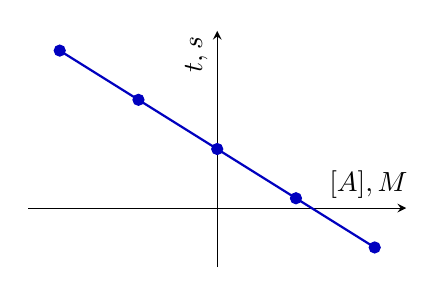
\begin{tikzpicture}
  \begin{axis}[
            axis lines=middle,
             enlargelimits=0.1,y=0.5cm/2, x=0.4cm,
%            xmin=0,
%            xmax=1.0,
%            ymin=0.01,
%            ymax=0.1,
            xtick=\empty,
            ytick=\empty,xtick distance=0.05,
            xlabel=$\text{ [A], M}$,
            ylabel=$\text{t, s }$,
            x label style={at={(axis description cs:0.9,0.45)},anchor=north},
    y label style={at={(axis description cs:0.5,.9)},rotate=90,anchor=south},
%             domain=\pgfkeysvalueof{/pgfplots/xmin}:(\pgfkeysvalueof{/pgfplots/xmax},
        ]
            \addplot [thick,draw=blue!75!black]{-1*x+3};
                         \addplot [blue!75!black, mark=*,  draw=none , samples=5 ]{-1*x+3};
	        \end{axis}
	        
\end{tikzpicture}\hspace{0.5cm}\vspace{-0.6cm}
%\begin{tikzpicture}
%  \begin{axis}[
%            axis lines=middle,
%             enlargelimits=0.1,y=0.35cm/3,
%    x=0.4cm,
%%            xmin=0,
%%            xmax=1.0,
%%            ymin=0.01,
%%            ymax=0.1,
%            xtick=\empty,
%            ytick=\empty,xtick distance=0.05,
%            xlabel=$\text{1/[A], 1/M}$,
%            ylabel=$\text{t, s   }$,
%            x label style={at={(axis description cs:0.9,0.45)},anchor=north},
%    y label style={at={(axis description cs:0.5,.9)},rotate=90,anchor=south},
%%             domain=\pgfkeysvalueof{/pgfplots/xmin}:(\pgfkeysvalueof{/pgfplots/xmax},
%        ]
%            \addplot [thick,draw=blue!75!black]{1*x+3};
%                         \addplot [blue!75!black, mark=*,  draw=none , samples=5 ]{1*x+3};
%	        \end{axis}
%	        
%\end{tikzpicture}
\end{center}

\end{question}
\begin{solution}
zeroth-order
\hspace{0.1cm}\end{solution}\stepcounter{numA}%%%%%%%%%%%%  



%%%%%%PROBLEM
\begin{question}[ID=\the\value{numA}]\SetQuestionProperties{section-title=\nameref{sec:units}}
The plot below resulting from integral method represent a perfect line with $r^2$=0.99. Indicate the order of the reaction.
\begin{center}
%\begin{tikzpicture}
%  \begin{axis}[
%            axis lines=middle,
%             enlargelimits=0.1,y=0.5cm/3, x=0.4cm,
%%            xmin=0,
%%            xmax=1.0,
%%            ymin=0.01,
%%            ymax=0.1,
%            xtick=\empty,
%            ytick=\empty,xtick distance=0.05,
%            xlabel=$\text{ [A], M}$,
%            ylabel=$\text{t, s }$,
%            x label style={at={(axis description cs:0.9,0.45)},anchor=north},
%    y label style={at={(axis description cs:0.5,.9)},rotate=90,anchor=south},
%%             domain=\pgfkeysvalueof{/pgfplots/xmin}:(\pgfkeysvalueof{/pgfplots/xmax},
%        ]
%            \addplot [thick,draw=blue!75!black]{-1*x+3};
%                         \addplot [blue!75!black, mark=*,  draw=none , samples=5 ]{-1*x+3};
%	        \end{axis}
%	        
%\end{tikzpicture}\hspace{0.5cm}\vspace{-0.6cm}
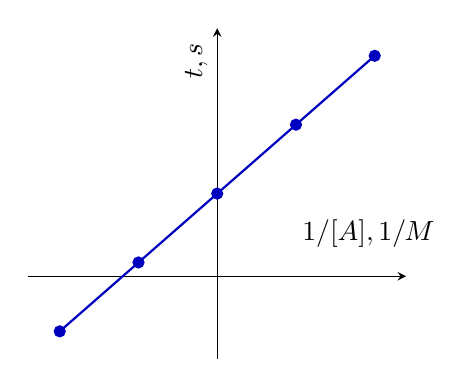
\begin{tikzpicture}
  \begin{axis}[
            axis lines=middle,
             enlargelimits=0.1,y=0.35cm/1,
    x=0.4cm,
%            xmin=0,
%            xmax=1.0,
%            ymin=0.01,
%            ymax=0.1,
            xtick=\empty,
            ytick=\empty,xtick distance=0.05,
            xlabel=$\text{1/[A], 1/M}$,
            ylabel=$\text{t, s   }$,
            x label style={at={(axis description cs:0.9,0.45)},anchor=north},
    y label style={at={(axis description cs:0.5,.9)},rotate=90,anchor=south},
%             domain=\pgfkeysvalueof{/pgfplots/xmin}:(\pgfkeysvalueof{/pgfplots/xmax},
        ]
            \addplot [thick,draw=blue!75!black]{1*x+3};
                         \addplot [blue!75!black, mark=*,  draw=none , samples=5 ]{1*x+3};
	        \end{axis}
	        
\end{tikzpicture}
\end{center}

\end{question}
\begin{solution}
second order
\hspace{0.1cm}\end{solution}\stepcounter{numA}%%%%%%%%%%%%  



%%%%%%PROBLEM
\begin{question}[ID=\the\value{numA}]\SetQuestionProperties{section-title=\nameref{sec:units}}
The plot below resulting from integral method represent a perfect line with $r^2$=0.99. Indicate the order of the reaction.
\begin{center}
%\begin{tikzpicture}
%  \begin{axis}[
%            axis lines=middle,
%             enlargelimits=0.1,y=0.5cm/3, x=0.4cm,
%%            xmin=0,
%%            xmax=1.0,
%%            ymin=0.01,
%%            ymax=0.1,
%            xtick=\empty,
%            ytick=\empty,xtick distance=0.05,
%            xlabel=$\text{ [A], M}$,
%            ylabel=$\text{t, s }$,
%            x label style={at={(axis description cs:0.9,0.45)},anchor=north},
%    y label style={at={(axis description cs:0.5,.9)},rotate=90,anchor=south},
%%             domain=\pgfkeysvalueof{/pgfplots/xmin}:(\pgfkeysvalueof{/pgfplots/xmax},
%        ]
%            \addplot [thick,draw=blue!75!black]{-1*x+3};
%                         \addplot [blue!75!black, mark=*,  draw=none , samples=5 ]{-1*x+3};
%	        \end{axis}
%	        
%\end{tikzpicture}\hspace{0.5cm}\vspace{-0.6cm}
\begin{tikzpicture}
  \begin{axis}[
            axis lines=middle,
             enlargelimits=0.1,y=0.35cm/1,
    x=0.4cm,
%            xmin=0,
%            xmax=1.0,
%            ymin=0.01,
%            ymax=0.1,
            xtick=\empty,
            ytick=\empty,xtick distance=0.05,
            xlabel=$\text{Ln[A]}$,
            ylabel=$\text{t, s   }$,
            x label style={at={(axis description cs:0.9,0.45)},anchor=north},
    y label style={at={(axis description cs:0.5,.9)},rotate=90,anchor=south},
%             domain=\pgfkeysvalueof{/pgfplots/xmin}:(\pgfkeysvalueof{/pgfplots/xmax},
        ]
            \addplot [thick,draw=blue!75!black]{-1*x+2};
                         \addplot [blue!75!black, mark=*,  draw=none , samples=5 ]{-1*x+2};
	        \end{axis}
	        
\end{tikzpicture}
\end{center}

\end{question}
\begin{solution}
first order
\hspace{0.1cm}\end{solution}\stepcounter{numA}%%%%%%%%%%%%  




%%%%%%PROBLEM
\begin{question}[ID=\the\value{numA}]\SetQuestionProperties{section-title=\nameref{sec:units}}
The following plots results from processing data by means of the integral method. Interpret the linear regressions and indicate the rate law.
\begin{center}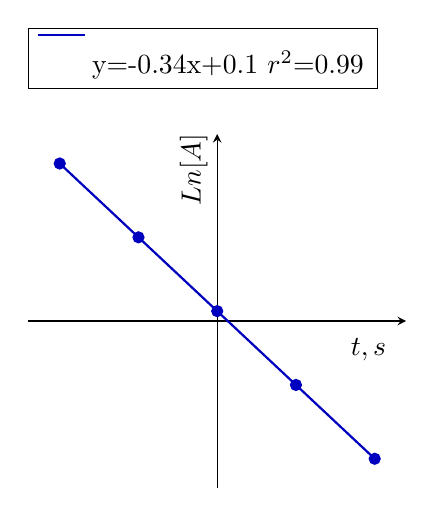
\begin{tikzpicture}
  \begin{axis}[
            axis lines=middle,legend style={at={(0.0,1.3)},anchor=north west} ,
             enlargelimits=0.1,y=0.5cm/4,
    x=0.4cm,
            xtick=\empty,
            ytick=\empty,xtick distance=0.05,
            xlabel=$\text{t, s}$,
            ylabel=$\text{Ln[A]}$,
            x label style={at={(axis description cs:0.9,0.45)},anchor=north},
    y label style={at={(axis description cs:0.5,.9)},rotate=90,anchor=south},
        ]
            \addplot [thick,draw=blue!75!black]{-3*x+1};      
                                \addlegendentry[shift={(0,0em)}]{y=-0.34x+0.1 $r^2$=0.99  };
                         \addplot [blue!75!black, mark=*,  draw=none , samples=5 ]{-3*x+1};
	        \end{axis}
	        
\end{tikzpicture}\end{center}
\end{question}
\begin{solution}
 $r=0.34[A]^1$, [A]$_0$=1.1M
\hspace{0.1cm}\end{solution}\stepcounter{numA}%%%%%%%%%%%%



%%%%%%PROBLEM
\begin{question}[ID=\the\value{numA}]\SetQuestionProperties{section-title=\nameref{sec:units}}
The following plots results from processing data by means of the integral method. Interpret the linear regressions and indicate the rate law.
\begin{center}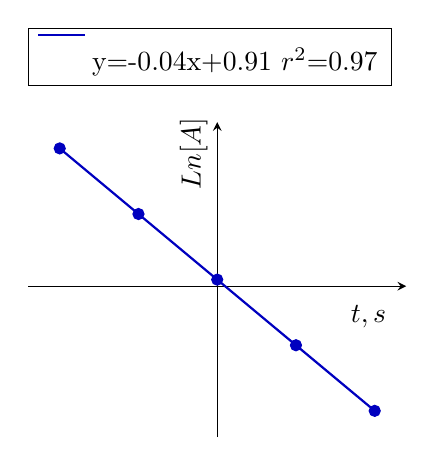
\begin{tikzpicture}
  \begin{axis}[
            axis lines=middle,legend style={at={(0.0,1.3)},anchor=north west} ,
             enlargelimits=0.1,y=0.5cm/6,
    x=0.4cm,
            xtick=\empty,
            ytick=\empty,xtick distance=0.05,
            xlabel=$\text{t, s}$,
            ylabel=$\text{Ln[A]}$,
            x label style={at={(axis description cs:0.9,0.45)},anchor=north},
    y label style={at={(axis description cs:0.5,.9)},rotate=90,anchor=south},
        ]
            \addplot [thick,draw=blue!75!black]{-4*x+1};      
                                \addlegendentry[shift={(0,0em)}]{y=-0.04x+0.91 $r^2$=0.97  };
                         \addplot [blue!75!black, mark=*,  draw=none , samples=5 ]{-4*x+1};
	        \end{axis}
	        
\end{tikzpicture}\end{center}
\end{question}
\begin{solution}
No rate maw can be deribed
\hspace{0.1cm}\end{solution}\stepcounter{numA}%%%%%%%%%%%%


%%%%%%PROBLEM
\begin{question}[ID=\the\value{numA}]\SetQuestionProperties{section-title=\nameref{sec:units}}
The following plots results from processing data by means of the integral method. Interpret the linear regressions and indicate the rate law.
\begin{center}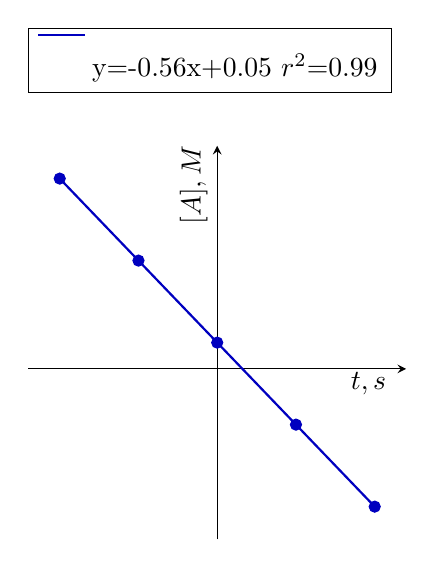
\begin{tikzpicture}
  \begin{axis}[
            axis lines=middle,legend style={at={(0.0,1.3)},anchor=north west} ,
             enlargelimits=0.1,y=0.5cm/6,
    x=0.4cm,
            xtick=\empty,
            ytick=\empty,xtick distance=0.05,
            xlabel=$\text{t, s}$,
            ylabel=$\text{  [A], M}$,
            x label style={at={(axis description cs:0.9,0.45)},anchor=north},
    y label style={at={(axis description cs:0.5,.9)},rotate=90,anchor=south},
        ]
            \addplot [thick,draw=blue!75!black]{-5*x+4};      
                                \addlegendentry[shift={(0,0em)}]{y=-0.56x+0.05 $r^2$=0.99  };
                         \addplot [blue!75!black, mark=*,  draw=none , samples=5 ]{-5*x+4};
	        \end{axis}
	        
\end{tikzpicture}\end{center}
\end{question}
\begin{solution}
 $r=0.56 $, [A]$_0$=0.05M
\hspace{0.1cm}\end{solution}\stepcounter{numA}%%%%%%%%%%%%


%%%%%%PROBLEM
\begin{question}[ID=\the\value{numA}]\SetQuestionProperties{section-title=\nameref{sec:units}}
Using the following data, calculate the order and rate constant and write down the rate law.
\begin{center}\begin{tabular}[t]{   c  c   }
\toprule
  $t$ ( s)	&$[A]$, (M) \\
\midrule
5&	0.952\\
10&	0.625\\
15&	0.465\\
20&	0.370\\
25&	0.308\\
35&	0.230\\
\bottomrule
\end{tabular}\end{center}
\end{question}
\begin{solution}
 $r=0.11[A]^2$, [A]$_0$=2M
\hspace{0.1cm}\end{solution}\stepcounter{numA}%%%%%%%%%%%%

%%%%%%PROBLEM
\begin{question}[ID=\the\value{numA}]\SetQuestionProperties{section-title=\nameref{sec:units}}
Using the following data, calculate the order and rate constant and write down the rate law.
\begin{center}\begin{tabular}[t]{   c  c   }
\toprule
  $t$ ( s)	&$[A]$, (M) \\
\midrule
0&	$9.90\times10^{-2}$\\
5&	$4.97\times10^{-2}$\\
10&	$3.32\times10^{-2}$\\
15&	$2.49\times10^{-2}$\\
20&	$1.66\times10^{-2}$\\
25&	$1.43\times10^{-2}$\\
\bottomrule
\end{tabular}\end{center}
\end{question}
\begin{solution}
 $r=2.45[A]^2$, [A]$_0$=0.13M
\hspace{0.1cm}\end{solution}\stepcounter{numA}%%%%%%%%%%%%




%%%%%%PROBLEM
\begin{question}[ID=\the\value{numA}]\SetQuestionProperties{section-title=\nameref{sec:units}}
Calculate the rate law for the following reaction using the given data:
\ce{2ClO2 +  2I^- -> 2ClO2^-    +  I2}
\begin{center}\begin{tabular}[t]{   c  c   }
\toprule
  $t$ ( s)	&$[\ce{ClO2}]$, (M) \\
\midrule
0&	$4.77\times10^{-4}$\\	
1&	$3.31\times10^{-4}$\\
2&	$3.91\times10^{-4}$\\
3&	$3.53\times10^{-4}$\\
5&	$2.89\times10^{-4}$\\
10&	$1.76\times10^{-4}$\\
30&	$2.40\times10^{-5}$\\
50&	$3.20\times10^{-6}$\\
\bottomrule
\end{tabular}\end{center}
\end{question}
\begin{solution}
 $r=0.098[\ce{ClO2}]$, [\ce{ClO2}]$_0$=$4.5\times 10^{-4}$M
\hspace{0.1cm}\end{solution}\stepcounter{numA}%%%%%%%%%%%%


	%%%%%%PROBLEM
\begin{question}[ID=\the\value{numA}]\SetQuestionProperties{section-title=\nameref{sec:units}}
Calculate the rate law for the following reaction using the given data: 
\ce{CH3COOCH3	+ OH^- -> CH3COO^-    +  CH3OH}
\begin{center}\begin{tabular}[t]{   c  c   }
\toprule
  $t$ ( s)	&$[\ce{CH3COOCH3}]$, (M) \\
\midrule
	0	&$1.00\times10^{-2}$\\
	3	&$7.40\times10^{-3}$\\
	4	&$6.83\times10^{-3}$\\
	5	&$6.34\times10^{-3}$\\
	10	&$4.63\times10^{-3}$\\
	20	&$3.04\times10^{-3}$\\
	30&$2.24\times10^{-3}$\\
\bottomrule
\end{tabular}\end{center}
\end{question}
\begin{solution}
 $r=11.51[\ce{CH3COOCH3}]^2$, [\ce{CH3COOCH3}]$_0$=$9.9\times 10^{-3}$M
\hspace{0.1cm}\end{solution}\stepcounter{numA}%%%%%%%%%%%%


	

		%%%%%%PROBLEM
\begin{question}[ID=\the\value{numA}]\SetQuestionProperties{section-title=\nameref{sec:units}}
Calculate the rate law for the following reaction using the given data: \ce{2NO2 -> 2NO    +  O2} 
\begin{center}\begin{tabular}[t]{   c  c   }
\toprule
  $t$ ( s)	&$[\ce{NO2}]$, (M) \\
\midrule
0&	$1.00\times10^{-2}$\\
60&	$6.83\times10^{-3}$\\
120&	$5.18\times10^{-3}$\\
180&	$4.18\times10^{-3}$\\
240&$3.50\times10^{-3}$\\
300&$	3.01\times10^{-3}$\\
360&	$2.64\times10^{-3}$\\
\bottomrule
\end{tabular}\end{center}
\end{question}
\begin{solution}
 $r=0.77[\ce{NO2}]^2$, [\ce{NO2}]$_0$=0.01M
\hspace{0.1cm}\end{solution}\stepcounter{numA}%%%%%%%%%%%%

			%%%%%%PROBLEM
\begin{question}[ID=\the\value{numA}]\SetQuestionProperties{section-title=\nameref{sec:units}}
Calculate the rate law for the following reaction using the given data: \ce{2HI -> H2    +  I2} 
\begin{center}\begin{tabular}[t]{   c  c   }
\toprule
  $t$ ( s)	&$[\ce{HI}]$, (M) \\
\midrule
		0	&	1\\
		1000	&	0.11\\
		2000	&	0.061\\
		3000	&	0.041\\
		4000	&	0.031\\
\bottomrule
\end{tabular}\end{center}
\end{question}
\begin{solution}
 $r=7.69\times 10^{-3}[\ce{HI}]^2$, [\ce{HI}]$_0$=0.7M
\hspace{0.1cm}\end{solution}\stepcounter{numA}%%%%%%%%%%%%	
		
		
				%%%%%%PROBLEM
\begin{question}[ID=\the\value{numA}]\SetQuestionProperties{section-title=\nameref{sec:units}}
Calculate the rate law for the following reaction using the given data: 
 \ce{H2    +  I2 ->	2HI} 
\begin{center}\begin{tabular}[t]{   c  c   }
\toprule
  $t$ ( s)	&$[\ce{H2}]$, (M) \\
\midrule
		0&	1\\
		1&	0.43	\\
		2&	0.27\\
		3&	0.20\\
		4&	0.16\\
\bottomrule
\end{tabular}\end{center}
\end{question}
\begin{solution}
 $r=7.69\times 10^{-3}[\ce{H2}]^2$, [\ce{H2}]$_0$=0.7M
\hspace{0.1cm}\end{solution}\stepcounter{numA}%%%%%%%%%%%%	
		
			
					%%%%%%PROBLEM
\begin{question}[ID=\the\value{numA}]\SetQuestionProperties{section-title=\nameref{sec:units}}
Calculate the rate law for the following reaction using the given data:\ce{C3H5    ->	C3H6} 
\begin{center}\begin{tabular}[t]{   c  c   }
\toprule
  $t$ ( s)	&$[\ce{C3H6}]$, (M) \\
\midrule
0&$1.5\times10^{-3}$\\
5&$1.24\times10^{-3}$\\
10&$1.0\times10^{-3}$\\
15&$0.83\times10^{-3}$\\
\bottomrule
\end{tabular}\end{center}
\end{question}
\begin{solution}
 $r=4.5\times 10^{-5}$, [\ce{C3H6}]$_0$=$1.48\times 10^{-3}$M
\hspace{0.1cm}\end{solution}\stepcounter{numA}%%%%%%%%%%%%			
		
			
		
					%%%%%%PROBLEM
\begin{question}[ID=\the\value{numA}]\SetQuestionProperties{section-title=\nameref{sec:units}}
Calculate the rate law for the following reaction using the given data:
 \ce{2P    +  Q -> W} 
\begin{center}\begin{tabular}[t]{   c  c   }
\toprule
  $t$ ( s)	&$[\ce{P}]$, (M) \\
\midrule
9&$1.077\times10^{-3}$\\
13&$1.068\times10^{-3}$\\
18&$1.055\times10^{-3}$\\
22&$1.046\times10^{-3}$\\
25&$1.039\times10^{-3}$\\
\bottomrule
\end{tabular}\end{center}
\end{question}
\begin{solution}
 $r=2.39\times 10^{-6}$, [\ce{P}]$_0$=$1.09\times 10^{-3}$M
\hspace{0.1cm}\end{solution}\stepcounter{numA}%%%%%%%%%%%%	




					%%%%%%PROBLEM
\begin{question}[ID=\the\value{numA}]\SetQuestionProperties{section-title=\nameref{sec:units}}
Calculate the rate law for the following reaction using the given data: \ce{2 O3    -> 3O2    } 
\begin{center}\begin{tabular}[t]{   c  c   }
\toprule
  $t$ ( h)	&$[\ce{O3}]$, (M) \\
\midrule
5&	0.952\\
10&	0.625\\
15&	0.465\\
20&	0.37\\
25&	0.308\\
35&0.23\\
\bottomrule
\end{tabular}\end{center}
\end{question}
\begin{solution}
 $r=0.109[\ce{O3}]^2$, [\ce{O3}]$_0$=1.99M
\hspace{0.1cm}\end{solution}\stepcounter{numA}%%%%%%%%%%%%	

	
	
					%%%%%%PROBLEM
\begin{question}[ID=\the\value{numA}]\SetQuestionProperties{section-title=\nameref{sec:units}}
Calculate the rate law for the following reaction using the given data: 
 \ce{2 X    -> Y + Z   } 
\begin{center}\begin{tabular}[t]{   c  c   }
\toprule
  $t$ ( s)	&$[\ce{ X}]$, (M) \\
\midrule
	5	&0.0990\\
	10&	0.0497\\
	15&	0.0332 \\
	20&	0.0249\\
	25&	0.0200\\
	30&	0.0166\\
	35	&0.0143\\
	40&0.0125 \\
\bottomrule
\end{tabular}\end{center}
\end{question}
\begin{solution}
 $r=1.99[\ce{ X}]^2$, [\ce{ X}]$_0$=6.15M
\hspace{0.1cm}\end{solution}\stepcounter{numA}%%%%%%%%%%%%	

	
	
	

	
{\raggedright\textsc{\textbf{Collision theory }}\par}

%%%%%%PROBLEM
\begin{question}[ID=\the\value{numA}]\SetQuestionProperties{section-title=\nameref{sec:units}}
For the energy profile below, indicate the activation energy and the reaction energy. Does this diagram corresponds to an exothermic or endothermic reaction?
\begin{center}
\begin{endiagram}[x-label-text=\footnotesize reaction coordinate, y-label-text={\footnotesize Enthalpy, kJ/mol}]
  \ENcurve{1,2,0}
  \ShowNiveaus[length=2,niveau={N1-1, N1-2,N1-3}]
  \node[below,xshift=4pt] at (N1-1) { } node[above,yshift=5pt] at (N1-1) {\small -20};
 \node[above] at (N1-2) {  } node[below,yshift=-5pt]  at (N1-2) {\small -5};
  \node[below,xshift=4pt] at (N1-3) {  } node[above,yshift=5pt] at (N1-3) {\small -35};
 \end{endiagram}\end{center}
\end{question}
\begin{solution}
$E_a=$15kJ/mol; $\Delta H=$-15kJ/mol; exothermic
\hspace{0.1cm}\end{solution}\stepcounter{numA}%%%%%%%%%%%% 
	
	 
%%%%%%PROBLEM
\begin{question}[ID=\the\value{numA}]\SetQuestionProperties{section-title=\nameref{sec:units}}
For the energy profile below, indicate the activation energy and the reaction energy. Does this diagram corresponds to an exothermic or endothermic reaction?
\begin{center}
\begin{endiagram}[x-label-text=\footnotesize reaction coordinate, y-label-text={\footnotesize Enthalpy, kJ/mol}]
  \ENcurve{1,2,1.5}
  \ShowNiveaus[length=2,niveau={N1-1, N1-2,N1-3}]
  \node[below,xshift=4pt] at (N1-1) { } node[above,yshift=5pt] at (N1-1) {\small -30};
 \node[above] at (N1-2) {  } node[below,yshift=-5pt]  at (N1-2) {\small -10};
  \node[below,xshift=4pt] at (N1-3) {  } node[above,yshift=5pt] at (N1-3) {\small -20};
 \end{endiagram}\end{center}
\end{question}
\begin{solution}
$E_a=$20kJ/mol; $\Delta H=$10kJ/mol; endothermic
\hspace{0.1cm}\end{solution}\stepcounter{numA}%%%%%%%%%%%%
	 
%%%%%%PROBLEM
\begin{question}[ID=\the\value{numA}]\SetQuestionProperties{section-title=\nameref{sec:units}}
Sketch an energy profile in which reactants are located at -10kJ/mol, the activation energy is 5kJ/mol and the energy of reaction is 10kJ/mol.
\end{question}
\begin{solution}
\begin{center}
\begin{endiagram}[x-label-text=\footnotesize reaction coordinate, y-label-text={\footnotesize Enthalpy, kJ/mol}]
  \ENcurve{1,2,0}
  \ShowNiveaus[length=2,niveau={N1-1, N1-2,N1-3}]
  \node[below,xshift=4pt] at (N1-1) { } node[above,yshift=5pt] at (N1-1) {\small -10};
 \node[above] at (N1-2) {  } node[below,yshift=-5pt]  at (N1-2) {\small -5};
  \node[below,xshift=4pt] at (N1-3) {  } node[above,yshift=5pt] at (N1-3) {\small 0};
 \end{endiagram}\end{center}\hspace{0.1cm}\end{solution}\stepcounter{numA}%%%%%%%%%%%%
	

%%%%%%PROBLEM
\begin{question}[ID=\the\value{numA}]\SetQuestionProperties{section-title=\nameref{sec:units}}
Sketch an energy profile in which reactants are located at -15kJ/mol, the activation energy is 10kJ/mol and the energy of reaction is -10kJ/mol.
\end{question}
\begin{solution}
\begin{center}
\begin{endiagram}[x-label-text=\footnotesize reaction coordinate, y-label-text={\footnotesize Enthalpy, kJ/mol}]
  \ENcurve{1,2,0}
  \ShowNiveaus[length=2,niveau={N1-1, N1-2,N1-3}]
  \node[below,xshift=4pt] at (N1-1) { } node[above,yshift=5pt] at (N1-1) {\small -15};
 \node[above] at (N1-2) {  } node[below,yshift=-5pt]  at (N1-2) {\small -5};
  \node[below,xshift=4pt] at (N1-3) {  } node[above,yshift=5pt] at (N1-3) {\small -25};
 \end{endiagram}\end{center}\hspace{0.1cm}\end{solution}\stepcounter{numA}%%%%%%%%%%%%

%%%%%%PROBLEM
\begin{question}[ID=\the\value{numA}]\SetQuestionProperties{section-title=\nameref{sec:units}}
Compare both energy profiles top and bottom and indicate:
\begin{inparaenum}[(a)]	
\item What reaction proceeds faster
\item What reaction exchanges more energy
\end{inparaenum}	
\begin{center}
\begin{endiagram}[x-label-text=\footnotesize reaction coordinate, y-label-text={\footnotesize Enthalpy, kJ/mol}]
  \ENcurve{1,2,1.5}
  \ShowNiveaus[length=2,niveau={N1-1, N1-2,N1-3}]
  \node[below,xshift=4pt] at (N1-1) { } node[above,yshift=5pt] at (N1-1) {\small -30};
 \node[above] at (N1-2) {  } node[below,yshift=12pt]  at (N1-2) {\small -10};
  \node[below,xshift=4pt] at (N1-3) {  } node[above,yshift=5pt] at (N1-3) {\small -20};
 \end{endiagram}\hspace{5cm}
 \begin{endiagram}[x-label-text=\footnotesize reaction coordinate, y-label-text={\footnotesize Enthalpy, kJ/mol}]
  \ENcurve{1,2,1.1}
  \ShowNiveaus[length=2,niveau={N1-1, N1-2,N1-3}]
  \node[below,xshift=4pt] at (N1-1) { } node[above,yshift=5pt] at (N1-1) {\small -40};
 \node[above] at (N1-2) {  } node[below,yshift=12pt]  at (N1-2) {\small -10};
  \node[below,xshift=4pt] at (N1-3) {  } node[above,yshift=5pt] at (N1-3) {\small -35};
 \end{endiagram}
 \end{center}
\end{question}
\begin{solution}
\begin{inparaenum}[(a)]	
\item top goes faster
\item top consumes more energy
\end{inparaenum}\hspace{0.1cm}\end{solution}\stepcounter{numA}%%%%%%%%%%%%

%%%%%%PROBLEM
\begin{question}[ID=\the\value{numA}]\SetQuestionProperties{section-title=\nameref{sec:units}}
The reaction energy of a process, going from reactants into products, is 10kJ/mol and its activation energy is 15kJ/mol. Calculate the reaction energy and the activation energy of the reverse process, starting from products and going to reactants. Is the direct reaction exothermic or endothermic. How about the reverse process?
\end{question}
\begin{solution}
$E_a=$5kJ/mol; $\Delta H=$-10kJ/mol; direct endothermic; reverse exothermic
\hspace{0.1cm}\end{solution}\stepcounter{numA}%%%%%%%%%%%%


%%%%%%PROBLEM
\begin{question}[ID=\the\value{numA}]\SetQuestionProperties{section-title=\nameref{sec:units}}
The rate constant for the gas-phase decomposition of \ce{N2O} 
has the following temperature dependence:
\begin{center}\ce{2N2O_{(g)} ->2N2_{(g)} + O2_{(g)}}\end{center}
has the following temperature dependence:
\begin{center}\begin{tabular}[t]{   c  c   }
\toprule
  $T$ ( K)	&$k$, ($s^{-1}$) \\
\midrule
1500&	$1.1\times 10^{-15}$\\
1400&	$1.4\times 10^{-13}$\\
1300&	$6.9\times 10^{-13}$\\
1200&$1.5\times 10^{-12}$\\
\bottomrule
\end{tabular}\end{center}
Indicate the reaction order, and compute the activation energy in (kJ/mol) and the frequency factor.
\end{question}
\begin{solution}
Order one; $E_a=$252.05kJ/mol; $A=5.52\times 10^{12}$ s$^{-1}$
\hspace{0.1cm}\end{solution}\stepcounter{numA}%%%%%%%%%%%%


%%%%%%PROBLEM
\begin{question}[ID=\the\value{numA}]\SetQuestionProperties{section-title=\nameref{sec:units}}
For the gas-phase reaction between hydrogen and iodine
 \begin{center}\ce{H2_{(g)}  + I2_{(g)} -> 2HI_{(g)} 		}\end{center}
the rate constant at 500K was found to be $9.36\times 10^{-7}$ 1/(M$\cdot$s) and the rate constant at 600K was found to be $5.69\times 10^{-4}$ 1/(M$\cdot$s). Calculate the activation energy in kJ/mol and the frequency factor of the reaction.
\end{question}
\begin{solution}
Order one; $E_a=$159.88kJ/mol; $A=4.73\times 10^{10}$ s$^{-1}$
\hspace{0.1cm}\end{solution}\stepcounter{numA}%%%%%%%%%%%%

%%%%%%PROBLEM
\begin{question}[ID=\the\value{numA}]\SetQuestionProperties{section-title=\nameref{sec:units}}
For the decomposition of dinitrogen pentoxide
 \begin{center}\ce{2N2O5_{(g)} -> 2N2O4_{(g)} + O2_{(g)}	 		}\end{center}
the rate constant at 500K is 345.43 s$^{-1}$ and at different temperature, the rate constant is 24.84 s$^{-1}$. Given that the activation energy of this reaction is 103.03 kJ/mol, calculate the second temperature value.
\end{question}
\begin{solution}
452K
\hspace{0.1cm}\end{solution}\stepcounter{numA}%%%%%%%%%%%%


%%%%%%PROBLEM
\begin{question}[ID=\the\value{numA}]\SetQuestionProperties{section-title=\nameref{sec:units}}
For a given reaction, when temperature increases from 100K to 200K, its rate constant triples. 
Calculate the activation energy for this process.
\end{question}
\begin{solution}
1.8kJ/mol
\hspace{0.1cm}\end{solution}\stepcounter{numA}%%%%%%%%%%%%


{\raggedright\textsc{\textbf{Reaction mechanisms }}\par}


%%%%%%PROBLEM
\begin{question}[ID=\the\value{numA}]\SetQuestionProperties{section-title=\nameref{sec:units}}
For the following elemental reaction steps indicate the molecularity and give the rate law:
  \begin{enumerate} [topsep=0pt, partopsep=1pt, label=(\alph*), leftmargin=0.5cm]	
\item \ce{N2O -> NO + O}   %molecularity=1; $r$=k[\ce{N2O}]
\item \ce{N2O + O -> N2 + O2}%molecularity=2; $r$=k[\ce{N2O}][\ce{O}]
\item \ce{2NO -> N2O2}%molecularity=2; $r$=k[\ce{NO}]
\item \ce{N2O2 + H -> N2O + HO}%molecularity=2; $r$=k[\ce{N2O2}][\ce{H}]
\end{enumerate}
\end{question}
\begin{solution}
  \begin{enumerate} [topsep=0pt, partopsep=1pt, label=(\alph*), leftmargin=0.5cm]	
\item  molecularity=1; $r$=k[\ce{N2O}]
\item  molecularity=2; $r$=k[\ce{N2O}][\ce{O}]
\item  molecularity=2; $r$=k[\ce{NO}]
\item  molecularity=2; $r$=k[\ce{N2O2}][\ce{H}]
\end{enumerate}
\hspace{0.1cm}\end{solution}\stepcounter{numA}%%%%%%%%%%%%

%%%%%%PROBLEM
\begin{question}[ID=\the\value{numA}]\SetQuestionProperties{section-title=\nameref{sec:units}}
The experimental rate law for the reaction of nitrogen monoxide and molecular oxygen given by the following reaction
  \begin{center}	\ce{2NO_{(g)} + O2_{(g)} -> 2NO2_{(g)}  	 		}\hfill r$^{Exp}$=k$^{Exp}$ [\ce{N2O}]$^2$[\ce{O2}]\end{center}
is second order with respect to dinitrogen oxide and first order with respect to oxygen. A plausible mechanism would be:
  \begin{center}(1)\hfill\ce{ NO_{(g)} + NO_{(g)} <=>[$k_1$][$k_{-1}$]     N2O2_{(g)}  }{   \hfill {} } \\
(2)\hfill\ce{$\textcolor{black}{\ce{N2O2_{(g)}}}$ + O2_{(g)} ->[$k_2$] 2NO2_{(g)}}{  \hfill(\small slow)\hfill } 
\end{center}
Calculate: 
\begin{inparaenum}[(a)]	
\item  the molecularity of each reaction step % (2;2)
\item  the rate law for each reaction step % ($0=k_1[\ce{NO}]^2-k_{-1}[\ce{N2O2}]$ ; $r_2=k_2[\ce{N2O2}][\ce{O2}]$		)
\item identify all intermediates %(\ce{N2O2})
\item justify whether the suggested mechanism is valid and if so give k$^{Exp}$ in terms of the rate constants in the mechanism % $\frac{k_2\cddot k_1}{k_{-1}}$
 \end{inparaenum}
\end{question}
\begin{solution}
\begin{inparaenum}[(a)]
\item   (2;2)
\item   $0=k_1[\ce{NO}]^2-k_{-1}[\ce{N2O2}]$ ; $r_2=k_2[\ce{N2O2}][\ce{O2}]$		 
\item  \ce{N2O2} 
\item  $\frac{k_2\cddot k_1}{k_{-1}}$
 \end{inparaenum}
\hspace{0.1cm}\end{solution}\stepcounter{numA}%%%%%%%%%%%%




%%%%%%PROBLEM
\begin{question}[ID=\the\value{numA}]\SetQuestionProperties{section-title=\nameref{sec:units}}
A possible mechanism for the reaction of nitrogen monoxide and molecular oxygen to produce nitrogen dioxide given by the following reaction
  \begin{center}	\ce{2NO_{(g)} + O2_{(g)} -> 2NO2_{(g)}  	 		}\hfill \end{center}
could be:
  \begin{center}(1)\hfill\ce{ NO_{(g)} + O2_{(g)} ->[$k_1$]    NO3_{(g)}  }{   \hfill(\small slow)\hfill } \\
(2)\hfill\ce{$\textcolor{black}{\ce{NO3_{(g)}}}$ + NO_{(g)} ->[$k_2$] 2NO2_{(g)}}{  \hfill(\small fast)\hfill } 
\end{center}
Calculate: 
\begin{inparaenum}[(a)]	
\item  the molecularity of each reaction step %  2;2 
\item  the rate law for each reaction step %   $r_1=k_1[\ce{NO}]^2[\ce{O2}]$; $r_2=k_2[\ce{NO3}][\ce{NO}]$		 
\item identify all intermediates % \ce{NO3} 
\item give the experimental rate law % $r^{Exp}\sim r^{slow} = k_1[\ce{NO}]^2[\ce{O2}]$
 \end{inparaenum}
\end{question}
\begin{solution}
\begin{inparaenum}[(a)]
\item     2; 2 
\item      $r_1=k_1[\ce{NO}]^2[\ce{O2}]$; $r_2=k_2[\ce{NO3}][\ce{NO}]$		 
\item  \ce{NO3} 
\item   $r^{Exp}\sim r^{slow} = k_1[\ce{NO}]^2[\ce{O2}]$
 \end{inparaenum}
\hspace{0.1cm}\end{solution}\stepcounter{numA}%%%%%%%%%%%%




\end{multicols*}

\newpage
\begin{answersenvironment}
\begin{minipage}[c]{1\textwidth}
\begin{localsize}{10}
{\Large \bf Answers}
\SetupExSheets{
  headings = inline-nr , % numbered and inline
  counter-format = qu) , % numbers 1) 2) ... 
}
%\printsolutions 
 %\printsolutions[byID={1,3,5,7,9,11,13,15,17,19,21,23,25,27,29,31,33,35,37}]
\end{localsize}
\end{minipage}\end{answersenvironment}
\end{document}

